\section{Details on Real-Data Examples}
\subsection{ICU Mortality Example}
\label{appendix:icu_details}

This appendix provides full details on how we constructed the ICU data subsets, prepared the analytic dataset, estimated the OBD, identified sign reversals, and computed bootstrap standard errors for all data subsets used in \cref{sec:real_example}. The analyses use the PhysioNet ICU cohort collected for the study of in-hospital mortality \citep{goldberger2000physiobank}. The raw cohort contains routine admission measurements for $3,997$ patients with known gender ($2,246$ women and $1,751$ men). We merge these records with the corresponding mortality outcomes and restrict attention to patients with complete information on the covariates used in the decomposition: age, ICU type, heart rate (HR), mean arterial pressure (MAP), temperature, urine output, and the indicator for in-hospital death. After removing observations with missing covariates, the final analytic dataset contains $3,429$ patients. All data subset definitions, model specifications, and statistical procedures described below are applied to this cleaned dataset.

\subsection*{Model specification}

For each data subset, we fit separate group-specific models of in-hospital mortality for men and for women. Let $g \in \{\text{men}, \text{women}\}$, let $Y$ be the indicator for in-hospital mortality, and let $X$ be the vector of admission covariates (heart rate, mean arterial pressure, temperature, urine output, age, and ICU type). For each group $g$, we fit an estimator $\hat{M}_g(X)$ of the conditional expectation $\E[Y \mid X, g]$ and use \cref{eq:OB_H_Counterfactual,eq:OB_K_Counterfactual}; see \cref{sec:ob_real}. We consider five model classes, specified as follows.

\textbf{Linear regression.} We take
\[
    \E[Y \mid X, g] \;=\; \alpha_{g} + X^{\top}\beta_{g},
\]
with the group-specific intercept $\alpha_{g}$ and slope $\beta_{g}$ estimated by ordinary least squares. Although $Y$ is binary, this linear probability model is the object to which the classical OBD applies and remains standard in applied work \citep{jann2008, edokaChangesCatastrophicHealth2017, sujin_LPM_OB, mweembaGapSelfRatedHealth2023}.

\textbf{Logistic regression.} Within each group, we standardize the covariates to zero mean and unit variance and fit a logistic regression of $Y$ on the standardized covariates with the default $L_2$ penalty.

\textbf{Neural network.} Within each group, we standardize the covariates and fit a two-hidden-layer fully-connected ReLU network with hidden widths $(32, 16)$, $L_2$ weight decay $10^{-4}$, the Adam optimizer \citep{kingma2015adam}, and max\_iter $=2000$.

\textbf{XGBoost.} We fit a gradient-boosted tree classifier with $250$ estimators, maximum depth $3$, learning rate $0.05$, row subsampling rate $0.9$, column subsampling rate $0.9$, $L_2$ leaf regularization $\lambda = 1.0$, histogram tree method, and the logistic (log-loss) objective.

\textbf{TabPFN.} We use a modern transformer-based tabular model, TabPFN \citep{hollmann2023tabpfn}\footnote{We note that TabPFN uses a custom license: \url{https://huggingface.co/Prior-Labs/tabpfn_2_6/blob/main/LICENSE}}, a pre-trained in-context classifier that maps a training set directly to a predictive distribution for $Y \mid X$. We use the publicly released v2.6 weights and use the v7.1.1 TabPFN code for inference. We run the model locally on a single NVIDIA A100 GPU with $80$~GB of vRAM.

For all five models, we take the predicted probability of in-hospital death as $\hat{M}_g(X)$ and estimate each NOBD counterfactual mean $\E_{g'}[\E_g[Y \mid X]]$ by the within-sample average $\frac{1}{|g'|}\sum_{i \in g'} \hat{M}_g(X_i)$.

\subsection*{Data subset construction}
The goal of this analysis was not to target any particular physiological pattern, but rather to explore systematically whether sign reversals arise in realistic data partitions that a practitioner might naturally encounter.

We constructed $139$ data subsets in total. These sets include: quartiles of each continuous admission vital (heart rate, MAP, temperature, urine output);
deciles of age; ICU-type specific cohorts; clinically motivated threshold subsets (HR $>100$, MAP $<65$, Temp $> 38^\circ$C, Urine $>1000$ mL); fifty random $50\%$ subsamples of the cohort; fifty random $30\%$ subsamples of the cohort.

For each data subset and each of the five models in our model class, we compute the decomposition under both reference groups, taking men and women in turn. We say that the explained or unexplained component sign flips in that data subset if its estimated value has opposite signs under the two reference choices. To assess whether such flips are robust to sampling variability, we next describe the bootstrap procedure we use to compute standard errors and $p$-values for each component.

\textbf{Bootstrap.}
For each data subset and each model, we compute bootstrap standard errors and $p$-values for the OBD components. The bootstrap procedure follows the standard Oaxaca--Blinder framework: men and women are resampled within group with replacement, preserving group sizes. For each bootstrap replication $b=1,\dots,B$, we re-fit the corresponding group-specific model and re-estimate the OBD components.

Let $\hat\theta$ denote any Oaxaca--Blinder component (for example, the explained component under the women reference model), and let $\hat\theta^{(1)},\dots,\hat\theta^{(B)}$ denote its bootstrap replicates. The bootstrap standard error and mean are
\[
    \widehat{\operatorname{se}}(\hat\theta)
    =
    \sqrt{
    \frac{1}{B-1}\sum_{b=1}^B
    \bigl(\hat\theta^{(b)} - \bar\theta\bigr)^2
    },
    \qquad
    \bar\theta = \frac{1}{B}\sum_{b=1}^B \hat\theta^{(b)}.
\]
$P$-values are computed using a normal approximation,
\[
    p = 2\left(1 - \Phi\left(\frac{|\hat\theta|}{\widehat{\operatorname{se}}(\hat\theta)}\right)\right).
\]

We say that a sign flip is significant at level $\alpha$ if, in addition to having opposite signs across reference groups, at least one of the two reference-specific estimates has $p < \alpha$. We summarize the total number of data subsets exhibiting any sign flip under each model in \cref{tab:flip_summary_main} in \cref{sec:real_example}. Here, \cref{tab:flip_summary_explained,tab:flip_summary_unexplained} below report the same counts separately for the explained and unexplained components.

We observed that empirically, the count of data subsets exhibiting a sign flip grows with model complexity for this particular data analysis. With the linear and logistic models showing the least amount of sign flips and only a couple remain significant at conventional thresholds. While the neural network and XGBoost show a substantial fraction of data subsets exhibits significant flips even at the $5\%$ level. Importantly, many of the flipped data subsets arise within the random subsamples, indicating that the OBD can yield unstable conclusions even when applied to simple resampled partitions of the same population. Several physiologically interpretable groups also displayed sign changes. The HR quartile two data subset examined in \cref{sec:real_example} is one such case, and serves as a concrete illustration of how these reversals can appear in clinically meaningful settings.

\begin{table}[!ht]
    \caption{Number of data subsets (out of $139$) exhibiting a sign flip in the explained component, by model. Columns $10\%$, $5\%$, and $1\%$ report the number of flipped data subsets that are significant at the corresponding level.}
    \label{tab:flip_summary_explained}
    \centering
    \small
    \begin{tabular}{lcccc}
    \toprule
    Model & Total flips & $10\%$ & $5\%$ & $1\%$ \\
    \midrule
    Linear      & 11 &  2 &  2 &  2 \\
    Logistic    &  9 &  2 &  2 &  1 \\
    Neural net  & 42 & 26 & 17 &  6 \\
    XGBoost     & 33 & 17 & 10 & 3 \\
    TabPFN      & 33 & 21 & 19 & 5 \\
    \bottomrule
    \end{tabular}
\end{table}

\begin{table}[!ht]
    \caption{Number of data subsets (out of $139$) exhibiting a sign flip in the unexplained component, by model. Columns $10\%$, $5\%$, and $1\%$ report the number of flipped data subsets that are significant at the corresponding level.}
    \label{tab:flip_summary_unexplained}
    \centering
    \small
    \begin{tabular}{lcccc}
    \toprule
    Model & Total flips & $10\%$ & $5\%$ & $1\%$ \\
    \midrule
    Linear      & 17 &  0 &  0 &  0 \\
    Logistic    & 21 &  0 &  0 &  0 \\
    Neural net  & 49 & 10 &  6 &  1 \\
    XGBoost     & 47 & 3 &  1 &  0 \\
    TabPFN      & 56 & 2 &  0 &  0 \\
    \bottomrule
    \end{tabular}
\end{table}

A substantial number of these sign reversals are significant at conventional thresholds, indicating that the instability documented in \cref{sec:real_example} is an inherent behavior of the OBD in this clinical dataset.


% \begin{table}[!t]
%     \centering
%     \caption{ICU Mortality Gap Decomposition for Data Subsets Exhibiting Sign Reversals. Standard errors in parentheses computed via bootstrap resampling with $1{,}000$ replications.  
%     P-values based on a normal approximation.  
%     Significance levels: * $p<0.10$, ** $p<0.05$, *** $p<0.01$.  
%     The decomposition separates the gender mortality gap (male minus female) into explained and unexplained components using the Oaxaca--Blinder method.  
%     Female Reference uses the model for females as the reference outcome structure; Male Reference uses the model for males.}
%     \label{tab:icu_mortality}
%     \scriptsize
%     \begin{tabular}{@{}lc*{5}{c}@{}}
%     \toprule
%     \multirow{2}{*}{Subset} &
%     \multirow{2}{*}{n} &
%     Gap &
%     \multicolumn{2}{c}{Female Reference} &
%     \multicolumn{2}{c}{Male Reference} \\
%     \cmidrule(lr){3-3} \cmidrule(lr){4-5} \cmidrule(lr){6-7}
%     & & (M–F) & Expl. & Unexp. & Expl. & Unexp. \\
%     \midrule
    
%     Age decile 1 & 344 & 0.027 & 0.002 & 0.025 & 0.036$^{*}$ & $-0.009$ \\
%     & & (0.033) & (0.009) & (0.033) & (0.019) & (0.030) \\[0.3em]
    
%     Age decile 2 & 347 & 0.004 & 0.023 & $-0.019$ & $-0.010$ & 0.015 \\
%     & & (0.033) & (0.021) & (0.041) & (0.014) & (0.036) \\[0.3em]
    
%     Age decile 4 & 372 & $-0.015$ & 0.012 & $-0.027$ & $-0.004$ & $-0.012$ \\
%     & & (0.032) & (0.013) & (0.035) & (0.017) & (0.037) \\[0.3em]
    
%     Age decile 5 & 344 & $-0.025$ & 0.010 & $-0.035$ & $-0.008$ & $-0.017$ \\
%     & & (0.039) & (0.016) & (0.039) & (0.022) & (0.042) \\[0.3em]
    
%     Age decile 9 & 325 & $-0.077$ & 0.001 & $-0.078$ & 0.001 & $-0.078$ \\
%     & & (0.048) & (0.023) & (0.049) & (0.013) & (0.049) \\[0.3em]
    
%     \textbf{HR quartile 2} & 816 & 0.035 & 0.021$^{***}$ & 0.014 & $-0.007$ & 0.042$^{*}$ \\
%     & & (0.023) & (0.007) & (0.025) & (0.011) & (0.025) \\[0.3em]
    
%     MAP quartile 0 & 877 & $-0.014$ & $-0.003$ & $-0.011$ & 0.004 & $-0.018$ \\
%     & & (0.026) & (0.009) & (0.026) & (0.008) & (0.026) \\[0.3em]
    
%     MAP quartile 1 & 840 & 0.024 & 0.036$^{***}$ & $-0.012$ & 0.011 & 0.013 \\
%     & & (0.022) & (0.012) & (0.027) & (0.008) & (0.022) \\[0.3em]
    
%     Urine quartile 0 & 859 & $-0.031$ & 0.007 & $-0.038$ & $-0.006$ & $-0.025$ \\
%     & & (0.027) & (0.009) & (0.027) & (0.007) & (0.027) \\[0.3em]
    
%     MAP $< 65$ & 697 & $-0.028$ & $-0.011$ & $-0.017$ & 0.002 & $-0.030$ \\
%     & & (0.029) & (0.012) & (0.029) & (0.008) & (0.029) \\[0.3em]
    
%     Temp $> 36.5$ & 267 & $-0.043$ & $-0.001$ & $-0.042$ & 0.008 & $-0.051$ \\
%     & & (0.047) & (0.025) & (0.050) & (0.019) & (0.046) \\[0.3em]
    
%     Urine $> 1000$ & 210 & 0.046 & $-0.014$ & 0.060 & 0.014 & 0.031 \\
%     & & (0.036) & (0.018) & (0.038) & (0.023) & (0.037) \\[0.3em]
    
%     Random 50\% \#6 & 1714 & 0.020 & 0.023$^{***}$ & $-0.003$ & 0.012$^{**}$ & 0.009 \\
%     & & (0.017) & (0.005) & (0.018) & (0.006) & (0.017) \\[0.3em]

%     Random 50\% \#21 & 1714 & 0.018 & 0.019$^{***}$ & $-0.001$ & 0.015$^{***}$ & 0.003 \\
%     & & (0.016) & (0.005) & (0.017) & (0.005) & (0.015) \\[0.3em]

%     Random 50\% \#28 & 1714 & 0.013 & 0.016$^{***}$ & $-0.004$ & 0.009$^{**}$ & 0.003 \\
%     & & (0.018) & (0.005) & (0.018) & (0.004) & (0.017) \\[0.3em]

%     Random 50\% \#30 & 1714 & 0.008 & 0.014$^{***}$ & $-0.006$ & 0.004 & 0.005 \\
%     & & (0.017) & (0.005) & (0.018) & (0.004) & (0.017) \\[0.3em]

%     Random 50\% \#34 & 1714 & 0.009 & 0.016$^{***}$ & $-0.007$ & 0.009$^{*}$ & 0.001 \\
%     & & (0.015) & (0.005) & (0.016) & (0.005) & (0.015) \\[0.3em]

%     Random 50\% \#39 & 1714 & 0.019 & 0.020$^{***}$ & $-0.001$ & 0.012$^{**}$ & 0.007 \\
%     & & (0.017) & (0.005) & (0.018) & (0.005) & (0.016) \\[0.3em]

%     Random 30\% \#0 & 1028 & 0.018 & 0.018$^{***}$ & $-0.001$ & 0.008 & 0.010 \\
%     & & (0.022) & (0.006) & (0.023) & (0.006) & (0.021) \\[0.3em]

%     Random 30\% \#5 & 1028 & 0.011 & 0.016$^{***}$ & $-0.005$ & 0.008 & 0.003 \\
%     & & (0.020) & (0.006) & (0.021) & (0.008) & (0.021) \\[0.3em]

%     Random 30\% \#17 & 1028 & 0.008 & 0.014$^{**}$ & $-0.006$ & 0.008 & 0.000 \\
%     & & (0.022) & (0.007) & (0.023) & (0.006) & (0.022) \\[0.3em]

%     Random 30\% \#18 & 1028 & 0.007 & 0.022$^{***}$ & $-0.015$ & 0.002 & 0.004 \\
%     & & (0.022) & (0.007) & (0.024) & (0.005) & (0.022) \\[0.3em]

%     Random 30\% \#20 & 1028 & 0.002 & 0.001 & 0.001 & 0.005 & $-0.003$ \\
%     & & (0.020) & (0.007) & (0.020) & (0.005) & (0.019) \\[0.3em]

%     Random 30\% \#24 & 1028 & 0.021 & 0.018$^{***}$ & 0.003 & $-0.007$ & 0.027 \\
%     & & (0.021) & (0.007) & (0.023) & (0.010) & (0.023) \\[0.3em]

%     Random 30\% \#31 & 1028 & 0.015 & 0.014$^{**}$ & 0.000 & 0.023$^{***}$ & $-0.009$ \\
%     & & (0.021) & (0.007) & (0.022) & (0.009) & (0.020) \\[0.3em]

%     Random 30\% \#37 & 1028 & 0.011 & 0.021$^{**}$ & $-0.011$ & 0.007 & 0.004 \\
%     & & (0.023) & (0.009) & (0.025) & (0.006) & (0.022) \\[0.3em]

%     Random 30\% \#43 & 1028 & 0.015 & 0.017$^{**}$ & $-0.002$ & 0.012$^{**}$ & 0.003 \\
%     & & (0.021) & (0.007) & (0.023) & (0.006) & (0.021) \\
    
%     \bottomrule
%     \end{tabular}
% \end{table}
    
\subsection*{HR quartile 2: results across models}
\label{appendix:hrq2}

\cref{sec:real_example} focuses on the HR quartile two data subset under the OBD. In \cref{tab:hrq2_bootstrap_models}, we report the corresponding decomposition under each of the five models in our model class. The linear, logistic, neural-network, and XGBoost results are obtained from the bootstrap procedure described above with $B = 1{,}000$ replications.

\begin{table}[!ht]
    \caption{OBD of the gender mortality gap in HR quartile two ($n = 816$), across all five models. The total gap is men's mean minus women's mean. Standard errors in parentheses are computed via bootstrap resampling with $1{,}000$ replications. $p$-values are based on a normal approximation (Wald test). Significance levels: * $p<0.10$, ** $p<0.05$, *** $p<0.01$.}
    \label{tab:hrq2_bootstrap_models}
    \centering
    \scriptsize
    \begin{tabular}{@{}lc*{4}{c}@{}}
    \toprule
    \multirow{2}{*}{Model} &
    \multirow{2}{*}{Gap (M--F)} &
    \multicolumn{2}{c}{Women reference} &
    \multicolumn{2}{c}{Men reference} \\
    \cmidrule(lr){3-4} \cmidrule(lr){5-6}
    & & Explained & Unexplained & Explained & Unexplained \\
    \midrule

    Linear
        & \makecell{$0.035$ \\ $(0.023)$}
        & \makecell{$0.021^{***}$ \\ $(0.007)$}
        & \makecell{$0.014$ \\ $(0.025)$}
        & \makecell{$-0.007$ \\ $(0.010)$}
        & \makecell{$0.042^{*}$ \\ $(0.025)$} \\[0.3em]

    Logistic
        & \makecell{$0.035$ \\ $(0.023)$}
        & \makecell{$0.026^{***}$ \\ $(0.009)$}
        & \makecell{$0.009$ \\ $(0.025)$}
        & \makecell{$-0.006$ \\ $(0.008)$}
        & \makecell{$0.041^{*}$ \\ $(0.024)$} \\[0.3em]

    Neural net
        & \makecell{$0.035$ \\ $(0.023)$}
        & \makecell{$0.001$ \\ $(0.024)$}
        & \makecell{$0.033$ \\ $(0.031)$}
        & \makecell{$0.053^{**}$ \\ $(0.022)$}
        & \makecell{$-0.018$ \\ $(0.025)$} \\[0.3em]

    XGBoost
        & \makecell{$0.035$ \\ $(0.023)$}
        & \makecell{$0.004$ \\ $(0.016)$}
        & \makecell{$0.031$ \\ $(0.025)$}
        & \makecell{$0.029^{**}$ \\ $(0.014)$}
        & \makecell{$0.006$ \\ $(0.021)$} \\[0.3em]

    TabPFN
        & \makecell{$0.035$ \\ $(0.023)$}
        & \makecell{$0.012$ \\ $(0.016$}                                                                                                                                                                                                                                                                              
        & \makecell{$0.023$ \\ $(0.026)$}
        & \makecell{$0.023^{*}$ \\ $(0.013)$} 
        & \makecell{$0.012$ \\ $(0.021)$} \\[0.3em]
    \bottomrule
    \end{tabular}
\end{table}

The linear and logistic OBD exhibit a consistent explained-component sign flip that is significant at the $1\%$ level, with very similar magnitudes: in both cases, the explained component is significantly positive under the women reference and flips to a small negative (non-significant) value under the men reference. The neural network and XGBoost both point to the men reference estimate being significantly positive at the $5\%$ level.

\cref{fig:hr_quartile2_hist} presents the histogram for the $816$ patients in HR quartile two, showing the distribution of mortality outcomes used in the linear probability models displayed in \cref{fig:sign_flip_overview} (left). \cref{tab:delta_mu_betas} shows the covariate mean differences and group-specific coefficients for HR quartile two that underlie the sign reversal documented in \cref{sec:real_example}.

\begin{figure}[!ht]
    \centerline{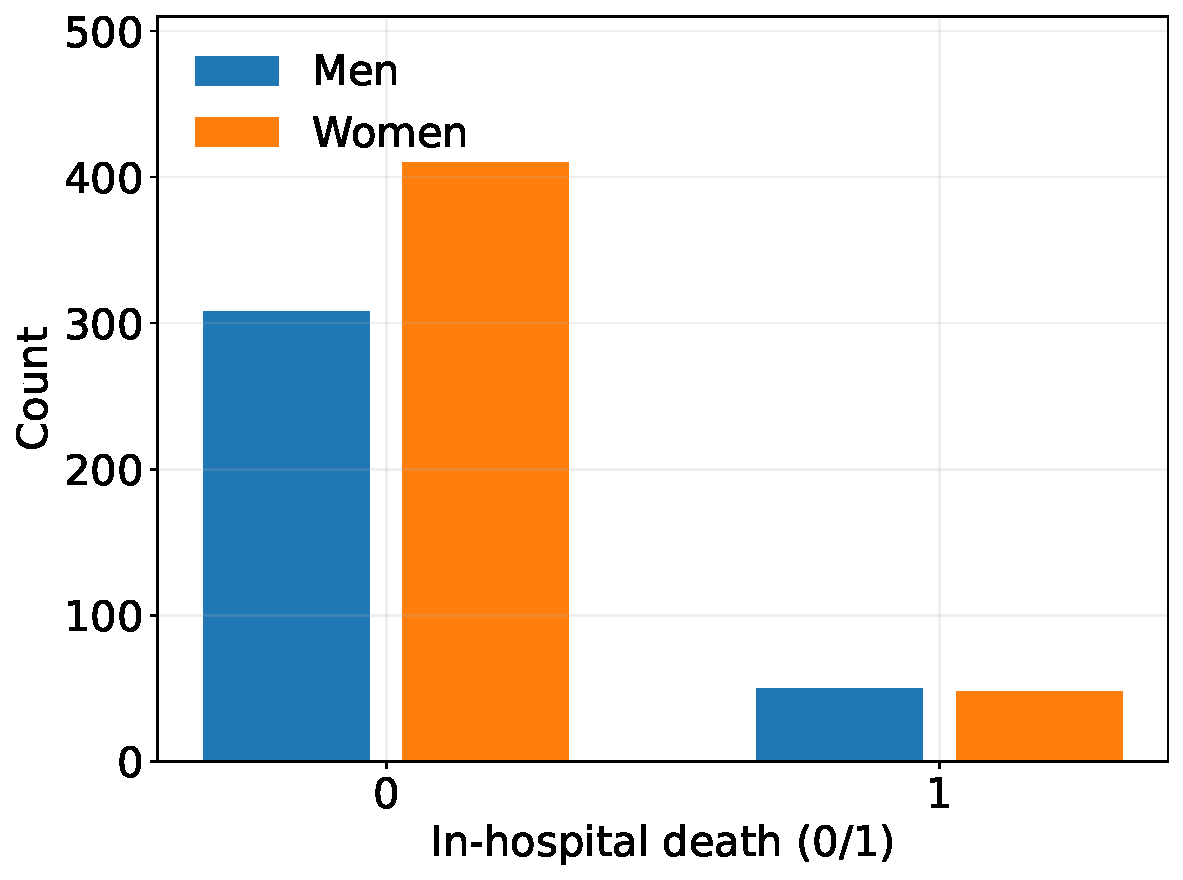
\includegraphics[width=0.5\linewidth]{Sections/Figures/hr_quartile2_mortality_y_hist.pdf}}
    \caption{Mortality outcome histogram for HR quartile two data subset.}
    \label{fig:hr_quartile2_hist}
\end{figure}

\begin{table}[!ht]
    \caption{Covariate mean differences and group-specific coefficients in HR quartile two. $\Delta\mu$ denotes the difference in covariate means between men and women within HR quartile two (men minus women). $\beta_{\text{Men}}$ and $\beta_{\text{Women}}$ are coefficients from group-specific linear probability models for in-hospital mortality.}
    \label{tab:delta_mu_betas}
    \centering
    \small
    \begin{tabular}{lrrr}
    \toprule
    Covariate 
    & $\Delta\mu$ 
    & $\beta_{\text{Men}}$ 
    & $\beta_{\text{Women}}$ \\
    \midrule
    Intercept & $0.0000$   & $1.1813$  & $-0.8515$ \\
    Age       & $3.8938$   & $-0.0000$ & $0.0039$ \\
    ICU Type  & $0.0095$   & $0.0173$  & $0.0116$ \\
    HR        & $0.4982$   & $-0.0026$ & $0.0056$ \\
    MAP       & $-0.6669$  & $0.0004$  & $0.0010$ \\
    Temp      & $0.3604$   & $-0.0230$ & $0.0028$ \\
    Urine     & $-39.8976$ & $-0.0001$ & $-0.0001$ \\
    \bottomrule
    \end{tabular}
\end{table}
    
\subsection{U.S.\ Labor Force Example}
\label{appendix:us_labor_force}
This appendix provides full details on how we constructed the U.S.\ labor force data subsets, prepared the analytic dataset, estimated the OBD, identified sign reversals, and computed bootstrap standard errors for all data subsets. 
The raw data come from the 2016 American Community Survey 1-Year Public Use Microdata Sample, which contains 1,625,282 observations.
We apply the same sample construction as \citet{bach2024heterogeneity}, who study the gender wage gap.
We restrict the sample to adults between the ages of 25 and 65, who were employed and at work as civilians, worked at least 35 hours per week, at least 50 weeks per year, and with both earnings and income above \$12,687.50 (which corresponds conservatively to an hourly wage of \$7.25).
The resulting sample contains 871,849 observations.

We purposely construct a large set of analyses to search for sign flips in different subsets of the data, comprising all combinations of the factors in \cref{tab:us_census_design}.

\begin{table}[!ht]
    \caption{Settings for sign flip search in the U.S.\ labor force dataset.}
    \label{tab:us_census_design}
    \centering
    \footnotesize
    \setlength{\tabcolsep}{4pt}
    \begin{tabular}{@{}llll@{}}
    \toprule
    Subset \( S \) & Outcome \( Y \) & Group (\( H, K \)) & Covariate (\(X\)) \\
    \midrule
    50 states + DC          & Income (\$)                & Sex (male, female)                   & Has Bachelor's degree (0/1) \\
    26 industries (NAICS 2) & Has health insurance (0/1) & Race (black, white)                  & Currently married (0/1)     \\
                            &                            & Nativity (native born, foreign born) & \\
    \bottomrule
    \end{tabular}
\end{table}

There are \( 77 \times 2 \times 3 \times 2 = 924\) combinations of these factors, each corresponding to a particular OBD that an analyst could compute.
We restrict our attention to cases where both groups have at least 50 observations within the subset (e.g., not computing a male-female OBD if there are fewer than 50 male and 50 female observations in that industry); \( | \Delta Y | > 0.01 \), and similarly for the explained and unexplained components.
These restrictions are intended to focus on cases where there is enough data to be informative,  and sign flips may be large in practical terms; they result in 355 comparisons.

For each comparison, we model the conditional expectation of the outcome as
\[
    \E[Y \mid X, g, s] \;=\; \alpha_{g,s} + X \beta_{g,s},
\]
where \( Y \) and \( X \) are the outcome and the covariate;
\( g \) indexes the group (i.e. male or female sex);
and \( s \) indicates a subset of the data (i.e., the state of Utah).
The parameters $(\alpha_{g,s},\beta_{g,s})$ are estimated using ordinary least squares.

Out of the 355 comparisons we examined, we found 0 cases where the explained component flipped signs and 1 case where the unexplained component flipped signs.
The sign flip occurs when comparing the explanatory power of education levels for explaining the foreign-native wage gap in Michigan, which we summarize in \cref{tab:us_census_flips}.
Regardless of the reference group, differences in education levels appear to explain most of the wage gap between the two groups.
However, taking the foreign-born population as the reference group, differences in how employers remunerate more educated workers seems to reduce the foreign-native gap ($p < 0.1$).
Taking the native-born population as the reference group, differences in remuneration seem to expand the gap, though the difference is statistically indistinguishable from zero.

\begin{table}[!ht]
    \caption{Outcome decomposition for subsets exhibiting sign reversals in the U.S.\ labor force. Standard errors in parentheses are computed via bootstrap resampling with $20{,}000$ replications. $p$-values are based on a normal approximation. Significance levels: * $p<0.10$, ** $p<0.05$, *** $p<0.01$.}
    \label{tab:us_census_flips}
    \centering
    \scriptsize
    \begin{tabular}{@{}lc*{5}{c}@{}}
    \toprule
    \multirow{2}{*}{Subset} &
    \multirow{2}{*}{Observations} &
    Gap &
    \multicolumn{2}{c}{Foreign Born Reference} &
    \multicolumn{2}{c}{Native Reference} \\
    \cmidrule(lr){3-3} \cmidrule(lr){4-5} \cmidrule(lr){6-7}
    State &  & (F–N) & Expl. & Unexp. & Expl. & Unexp. \\
    \midrule
    
    Michigan & 25,724 & 0.117$^{***}$ & 0.148$^{***}$  & \(-0.032\)$^{*}$ & 0.101$^{***}$ & 0.016   \\
             &        & (0.019)       & (0.011)        & (0.017)          & (0.007)       & (0.017) \\ [0.3em]
    \bottomrule
    \end{tabular}    
\end{table}
